% gm-15-NormalDistribution.tex

\documentclass[xcolor=dvipsnames]{beamer}

\usepackage{tikz}
\usepackage{cancel}
\renewcommand{\CancelColor}{\color{red}}
\usepackage{graphicx}
\usepackage{wrapfig}
\usepackage{colortbl}
\usepackage{color}
\usepackage{alltt}
\renewcommand*{\thefootnote}{\fnsymbol{footnote}}
\definecolor{myblue}{rgb}{0.8,0.85,1}

\mode<presentation>
{
  \usetheme{Warsaw}
  \setbeamercovered{transparent}
}
% \usecolortheme[named=OliveGreen]{structure}
\setbeamertemplate{navigation symbols}{} 
\setbeamertemplate{blocks}[rounded][shadow=true] 

% this is for overlaying math symbols, see https://tex.stackexchange.com/questions/12895/overlay-symbol-with-another
\def\qeq{\mathrel{%
    \mathchoice{\QEQ}{\QEQ}{\scriptsize\QEQ}{\tiny\QEQ}%
}}
\def\QEQ{{%
    \setbox0\hbox{$\longrightarrow$}%
    \rlap{\hbox to \wd0{\hss/\hss}}\box0
  }}

\newcounter{expls}
\setcounter{expls}{0}
\newcommand{\beispiel}[1]{\refstepcounter{expls}\textbf{Example \arabic{expls}: #1.}}

\newcounter{exercise}
\setcounter{exercise}{0}
\newcommand{\ubung}[0]{\refstepcounter{exercise}\textbf{Exercise \arabic{exercise}: }}

\newif\ifBCITCourse
\BCITCoursetrue
% \BCITCoursefalse
\newif\ifWhichCourse
\WhichCoursetrue
\WhichCoursefalse
\ifBCITCourse
\ifWhichCourse
\newcommand{\CourseName}{Technical Mathematics for Food Technology}
\newcommand{\CourseNumber}{MATH 1441}
\newcommand{\CourseInst}{BCIT}
\else
\newcommand{\CourseName}{Technical Mathematics for Geomatics}
\newcommand{\CourseNumber}{MATH 1511}
\newcommand{\CourseInst}{BCIT}
\fi
\else
\newcommand{\CourseName}{Philosophy and Literature}
\newcommand{\CourseNumber}{PHIL 375}
\newcommand{\CourseInst}{UBC}
\fi

\title{Normal Distribution}
\subtitle{{\CourseNumber}, BCIT}

\author{\CourseName}

\date{November 22, 2017}

\begin{document}

\begin{frame}
  \titlepage
\end{frame}

\begin{frame}
  \frametitle{Probabilities}
\alert{Probabilities} are positive real numbers that add up to 1. For example,
the probabilities for heads and tails on a coin flip may be
\begin{equation}
  \label{eq:veejooni}
  P(X=H)=0.5\mbox{ and }P(X=T)=0.5
\end{equation}
If you flip two coins, what are the probabilities for getting two
heads $(X=2)$, one head(s) $(X=1)$, or none $(X=0)$?
\end{frame}

\begin{frame}
  \frametitle{Binomial Probabilities I}
It turns out that order matters, so that
\begin{equation}
  \label{eq:eijietha}
  P(X=2)=\frac{1}{3},P(X=1)=\frac{1}{3},P(X=0)=\frac{1}{3}
\end{equation}
is incorrect, while the correct distribution is
\begin{equation}
  \label{eq:eepuneeb}
  P(X=2)=\frac{1}{4},P(X=1)=\frac{1}{2},P(X=0)=\frac{1}{4}
\end{equation}
because $P(X=1)=P(\mbox{HT})+P(\mbox{TH})=1/4+1/4=1/2$.
\end{frame}

\begin{frame}
  \frametitle{Binomial Probabilities II}
Here is the formula for a \alert{binomial} setup with $n$ trials (for example,
$n=2$ coin tosses), probability of success $p$ (for example, $p=0.5$ for the
probability of heads), and $x$ number of successes,
\begin{equation}
  \label{eq:iedohdah}
  P(X=x)=\frac{n!}{(n-x)!x!}p^{x}(1-p)^{n-x}
\end{equation}
where $0!=1$ and $(n+1)!=n!(n+1)$, for example
$4!=1\cdot{}2\cdot{}3\cdot{}4$ (say ``four factorial''). $X$ is a
\alert{random variable}, the number that the random process spits out.
\end{frame}

\begin{frame}
  \frametitle{Binomial Probabilities III}
Here are the binomial probabilities for $n=6$. One way to
conceptualize these numbers is by looking at Pascal's Triangle (next
slide). 
  \begin{figure}[h]
    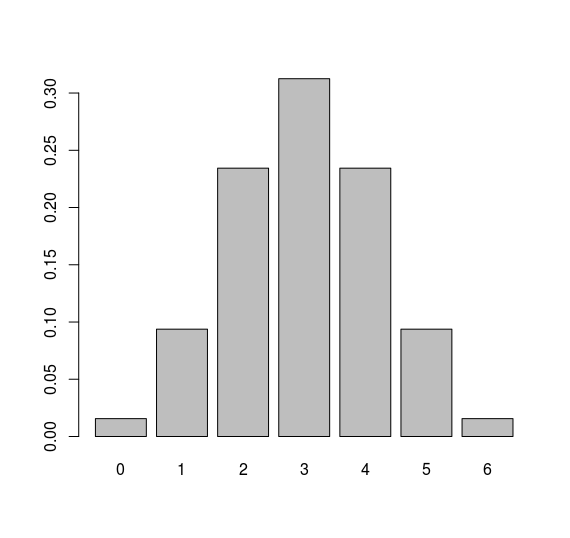
\includegraphics[scale=.5]{./binomial1.png}
  \end{figure}
\end{frame}

\begin{frame}
  \frametitle{Pascal's Triangle}
\begin{tikzpicture}
\foreach \n in {0,...,7} {
  \foreach \k in {0,...,\n} {
    \node at (\k-\n/2,-\n) {$\binom{\n}{\k}$};
  }
}
\end{tikzpicture}
\end{frame}

\begin{frame}
  \frametitle{Binomial Probabilities IV}
Binomial probabilities are difficult to calculate for high numbers. We
approximate the binomial distribution with the \alert{normal distribution}.
Compare the binomial distribution for $n=20$ with the normal
distribution.
  \begin{figure}[h]
    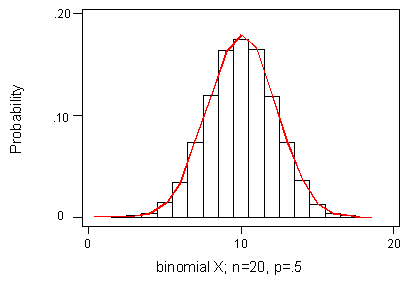
\includegraphics[scale=.5]{./binnorm.png}
  \end{figure}
\end{frame}

\begin{frame}
  \frametitle{Approximating the Binomial Distribution I}
For large numbers, even high-powered computers cannot calculate the
binomial probabilities. We use the normal distribution to approximate
the binomial distribution. Here is an example: if you roll a die 600
times, what is the probability of rolling a six fewer than 80 times? It
would take very long to calculate this probability using the binomial
distribution formula! We use the normal distribution with $\mu=np$ and
$\sigma=\sqrt{np(1-p)}$ instead. We make a \alert{continuity
  correction} and ask ourselves, what is the probability for the
$x$-score to be 79.5 or less for this normal distribution?
\begin{equation}
  \label{eq:oolojuth}
  z=\frac{x-\mu}{\sigma}=\frac{79.5-100}{9.1287}\approx{}-2.25
\end{equation}
The corresponding $p$-value is 0.0122. There is only a 1.22\%
probability that you will roll fewer than 80 sixes in 600 rolls.
\end{frame}

\begin{frame}
  \frametitle{Approximating the Binomial Distribution II}
Continuity correction means that when we approximate a whole number $m$
using the continuous normal distribution, we use the interval
$[m-0.5,m+0.5]$ to represent this whole number. ``Fewer than 80,'' for
example, is translated for the approximation as ``less than 79.5.''
``Fewer than or equal to 80'' is translated as ``less than 80.5.''

Conventionally, it is only acceptable to approximate the binomial
distribution by the normal distribution if $np\geq{}5$ and
$nq\geq{}5$. Otherwise, the binomial and the normal distribution are
too far apart to provide a useful approximation.
\end{frame}

\begin{frame}
  \frametitle{Normal Distribution}
There is not just one normal distribution. There are infinitely many,
characterized by their \alert{mean $\mu$} and their \alert{standard deviation
$\sigma$}. The formula for the normal distribution is
\begin{equation}
  \label{eq:aitoolah}
  f(x)=\frac{1}{\sigma\sqrt{2\pi}}e^{-(x-\mu)^{2}/(2\sigma^{2})}
\end{equation}
The area under the curve tells us something about the probability of
values in the intervals in which we are interested.
  \begin{figure}[h]
    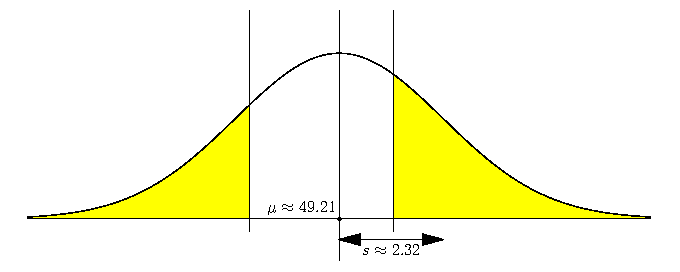
\includegraphics[scale=.4]{./qfour.png}
  \end{figure}
\end{frame}

\begin{frame}
  \frametitle{Z Scores}
To calculate the area under the curve, we carry around a piece of
paper with all the values for the \alert{standard normal distribution}
and then convert to the normal distribution with the relevant $\mu$
and $\sigma$. The value for the normal distribution is called the
\alert{$x$-score} and its associate value for the standard normal distribution
is called the \alert{$z$-score}. Travel back and forth using the following
formula,
\begin{equation}
  \label{eq:uotoogoo}
  z=\frac{x-\mu}{\sigma}
\end{equation}
\end{frame}

\begin{frame}
  \frametitle{Normal Distribution Example}
Here is an example. Men's heights are normally distributed with mean
$\mu=69.5$ inches and standard deviation $\sigma=2.4$ inches. What
percentage of the male population is taller than six feet (72 inches)?
Find the $z$-score, using the formula
\begin{equation}
  \label{eq:igutheib}
  z=\frac{x-\mu}{\sigma}=\frac{72-69.5}{2.4}\approx{}1.04
\end{equation}
Use your $z$-score table to find the corresponding \alert{$p$-value},
which is the area to the left of the $z$-score for the standard normal
distribution. In this case the $p$-value is $0.8508$. This represents
the percentage of the male population that is \emph{shorter} than 72
inches. The answer to our question is therefore, 14.92\% of men are
taller than six feet.
\end{frame}

\begin{frame}
  \frametitle{Approximating Binomial Probabilities I}
Here is the formula for a \alert{binomial} setup with $n$ trials (for example,
$n=2$ coin tosses), probability of success $p$ (for example, $p=0.5$ for the
probability of heads), and $x$ number of successes,
\begin{equation}
  \label{eq:iedohdah}
  P(X=x)=\frac{n!}{(n-x)!x!}p^{x}(1-p)^{n-x}
\end{equation}
where $0!=1$ and $(n+1)!=n!(n+1)$, for example
$4!=1\cdot{}2\cdot{}3\cdot{}4$ (say ``four factorial''). $X$ is a
\alert{random variable}, the number that the random process spits out.
\end{frame}

\begin{frame}
  \frametitle{Approximating Binomial Probabilities II}
Here are the binomial probabilities for $n=6$. One way to
conceptualize these numbers is by looking at Pascal's Triangle (next
slide). 
  \begin{figure}[h]
    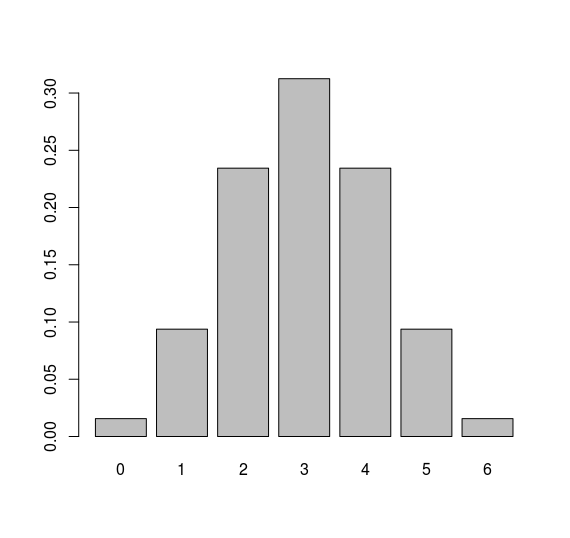
\includegraphics[scale=.5]{./binomial1.png}
  \end{figure}
\end{frame}

\begin{frame}
  \frametitle{Pascal's Triangle}
\begin{tikzpicture}
\foreach \n in {0,...,7} {
  \foreach \k in {0,...,\n} {
    \node at (\k-\n/2,-\n) {$\binomialCoefficient{\n}{\k}$};
  }
}
\end{tikzpicture}
\end{frame}

\begin{frame}
  \frametitle{Approximating Binomial Probabilities III}
Binomial probabilities are difficult to calculate for high numbers. We
approximate the binomial distribution with the \alert{normal distribution}.
Compare the binomial distribution for $n=10$ with the normal
distribution.
  \begin{figure}[h]
    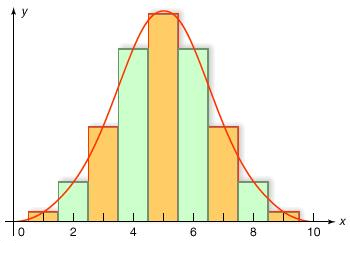
\includegraphics[scale=.5]{./binnorm1_ed.jpg}
  \end{figure}
\end{frame}

\begin{frame}
  \frametitle{Normal Distribution}
  The normal probabilities distribution is a \alert{continuous}
  probabilities distribution. There is not just one normal
  distribution. There are infinitely many, characterized by their
  \alert{mean $\mu$} and their \alert{standard deviation $\sigma$}.
  The formula for the normal distribution is
  \begin{equation}
    \label{eq:aitoolah}
    f(x)=\frac{1}{\sigma\sqrt{2\pi}}e^{-(x-\mu)^{2}/(2\sigma^{2})}
  \end{equation}
  \begin{figure}[h]
    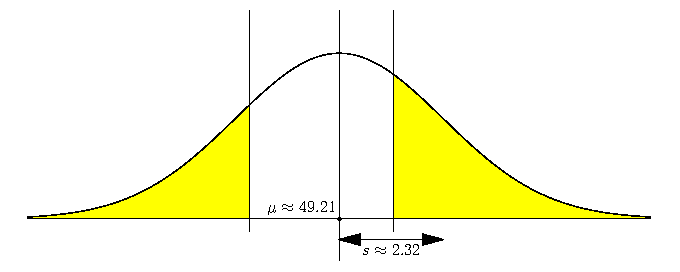
\includegraphics[scale=.4]{./qfour.png}
  \end{figure}
\end{frame}

\begin{frame}
  \frametitle{Z Scores}
  To calculate the area under the curve, we carry around a piece of
  paper with all the values for the \alert{standard normal
    distribution} and then convert to the normal distribution with the
  relevant $\mu$ and $\sigma$. The value for the normal distribution
  is called the \alert{$x$-score} and its associate value for the
  standard normal distribution is called the \alert{$z$-score}. Travel
  back and forth using the following formula,
  \begin{equation}
    \label{eq:uotoogoo}
    z=\frac{x-\mu}{\sigma}
  \end{equation}
\end{frame}

\begin{frame}
  \frametitle{Normal Distribution Example Question}
  \beispiel{Men's Heights} The height of adult men is normally
  distributed with mean $\mu=69.5$ inches and standard deviation
  $\sigma=2.4$ inches. What percentage of the adult male population is
  taller than six feet (72 inches)? 
\end{frame}

\begin{frame}
  \frametitle{Normal Distribution Example Answer}
  Find the $z$-score, using the formula
  \begin{equation}
    \label{eq:igutheib}
    z=\frac{x-\mu}{\sigma}=\frac{72-69.5}{2.4}\approx{}1.04
  \end{equation}
  Use your $z$-score table to find the corresponding
  \alert{$p$-value}, which is the area to the left of the $z$-score
  for the standard normal distribution. In this case the $p$-value is
  $0.8508$. This represents the percentage of the male population that
  is \emph{shorter} than 72 inches. The answer to our question is
  therefore, 14.92\% of men are taller than six feet.
\end{frame}

\begin{frame}
  \frametitle{Normal Distribution Exercises I}
{\ubung} Find the area under the curve for the following sets of
$z$-scores. 
\begin{equation}
  \label{eq:deapheph}
\{z|z\leq{}-1.72\}  
\end{equation}
\begin{equation}
  \label{eq:taedaiga}
\{z|1.96<{}z\}  
\end{equation}
\begin{equation}
  \label{eq:ahraefis}
\{z|-1.55\leq{}z\leq{}-0.81\}
\end{equation}
\end{frame}

\begin{frame}
  \frametitle{Normal Distribution Exercises II}
{\ubung} Find the area under the curve for the
following sets of $x$-scores. 
\begin{equation}
  \label{eq:aequaixe}
\{x|x\leq{}83\},\mu=100,\sigma=15
\end{equation}
\begin{equation}
  \label{eq:oocohdau}
\{x|0.44<x\},\mu=0.5,\sigma=0.2  
\end{equation}
\begin{equation}
  \label{eq:aethohph}
\{x|800\leq{}x\leq{}1200\},\mu=911,\sigma=121
\end{equation}
\end{frame}

\begin{frame}
  \frametitle{Normal Distribution Exercises III}
{\ubung} The time it takes a student to solve a particular math problem is
normally distributed with $\mu=3$ minutes and $27$ seconds and a
standard deviation of $\sigma=59$ seconds. How many students finish
the math problem between 3 and 4 minutes?
\end{frame}

\begin{frame}
  \frametitle{Normal Distribution Exercises IV}
  {\ubung} Scores on a certain intelligence test for children between
  ages 13 and 15 years are approximately normally distributed with
  $\mu=106$ and $\sigma=15$.
  \begin{enumerate}
  \item What proportion of children aged 13 to 15 years old have
    scores on this test above 88?
  \item Enter the score which marks the lowest 30 percent of the
    distribution.
  \item Enter the score which marks the highest 15 percent of the
    distribution.
  \end{enumerate}
When you want to find an $x$-score given a $p$-value, you need to use
your table in reverse and then find the $x$-score given the $z$-score
from the table by using the formula
\begin{equation}
  \label{eq:aedecaba}
  x=z\cdot\sigma+\mu
\end{equation}
\end{frame}
\begin{frame}
  \frametitle{Approximating Binomial Probabilities Example I}
  For large numbers, even high-powered computers cannot calculate the
  binomial probabilities. We use the normal distribution to
  approximate the binomial distribution. 

\bigskip

  \beispiel{Die Rolls} If you roll a die 600 times, what is the
  probability of rolling a six fewer than 80 times? 

\bigskip

  It would take very long to calculate this probability using the
  binomial distribution formula! We use the normal distribution with
  $\mu=np$ and $\sigma=\sqrt{np(1-p)}$ instead. 

\bigskip

  Conventionally, it is only acceptable to approximate the binomial
  distribution by the normal distribution if $np\geq{}5$ and
  $nq\geq{}5$. Otherwise, the binomial and the normal distribution are
  too far apart to provide a useful approximation.
\end{frame}

\begin{frame}
  \frametitle{Approximating Binomial Probabilities Example II}
  We need to make a \alert{continuity correction} and ask ourselves,
  what is the probability for the $x$-score to be 79.5 or less for
  this normal distribution?
  \begin{equation}
    \label{eq:oolojuth}
    z=\frac{x-\mu}{\sigma}=\frac{79.5-100}{9.1287}\approx{}-2.25
  \end{equation}
  The corresponding $p$-value is 0.0122. There is only a 1.22\%
  probability that you will roll fewer than 80 sixes in 600 rolls.
\end{frame}

\begin{frame}
  \frametitle{Continuity Correction}
  % Continuity correction means that when we approximate a whole number
  % $m$ using the continuous normal distribution, we use the interval
  % $[m-0.5,m+0.5]$ to represent this whole number. ``Fewer than 80,''
  % for example, is translated for the approximation as ``less than
  % 79.5.'' ``Fewer than or equal to 80'' is translated as ``less than
  % 80.5.''
  \begin{figure}[h]
    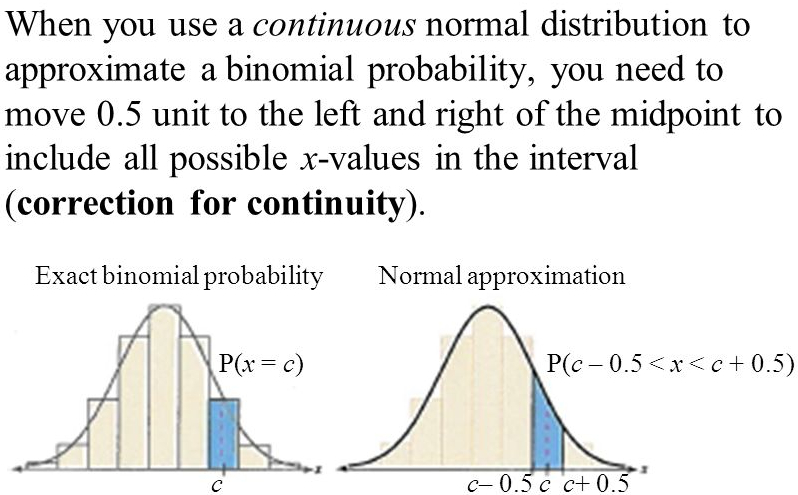
\includegraphics[scale=.5]{./contcorr_ed1.jpg}
  \end{figure}
\end{frame}

\begin{frame}
  \frametitle{Binomial Approximation Exercise}
{\ubung} 29\% of a country's population is blue-eyed. What is the
probability that a random sample of 1,000 persons contains between 200
and 300 blue-eyed persons? Approximate the binomial distribution by
the normal distribution. Calculate $\mu=np$ and
$\sigma=\sqrt{np(1-p)}$ for this normal distribution after checking
the conditions $np\geq{}5,n(1-p)\geq{}5$. Then calculate the
$z$-scores for the $x$-scores $x=199.5$ and $x=300.5$. Lastly,
determine the area under the curve between these $z$-scores. Provide a
complete sentence to answer the question.
\end{frame}

\begin{frame}
  \frametitle{Word Problems I}
  The national mortality rate for a particular type of heart surgery
  is 12\%, so you would expect six deaths per 50 operations. You are a
  health administrator, and one of your doctors has had eleven deaths
  in 72 operations. Should you fire her? What is the probability that
  an average surgeon (whose mortality rate is the national average)
  will have twelve or more deaths in 72 operations?

  \bigskip

  You desperately need a person with blood type AB (incidence in
  Canada: 3\%). If there are 49 people in the room, what is the
  probability that at least one of them is AB?
\end{frame}

\begin{frame}
  \frametitle{Word Problems I}
The national mortality rate for a particular type of heart surgery
is 12\%, so you would expect six deaths per 50 operations. You are a
health administrator, and one of your doctors has had eleven deaths in
72 operations. Should you fire her? What is the probability that an
average surgeon (whose mortality rate is the national average) will
have twelve or more deaths in 72 operations?

\bigskip

You desperately need a person with blood type AB (incidence in
Canada: 3\%). If there are 49 people in the room, what is the
probability that at least one of them is AB?
\end{frame}

\begin{frame}
  \frametitle{Word Problems II}
  \begin{figure}[h]
    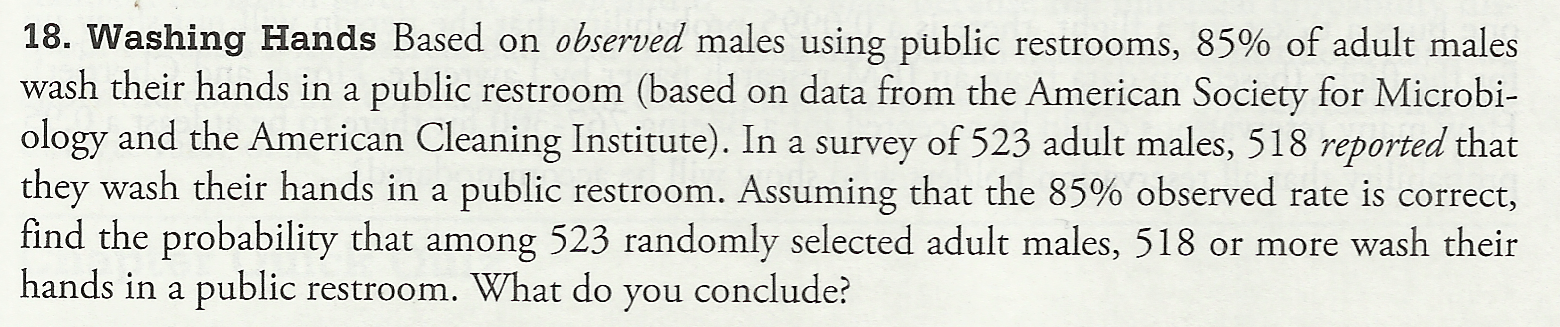
\includegraphics[scale=.7]{./triola1.png}
  \end{figure}
  \begin{figure}[h]
    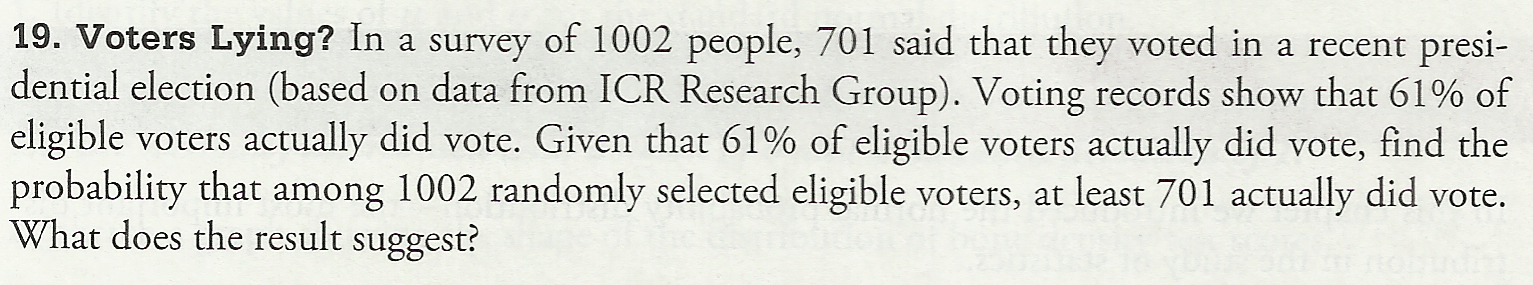
\includegraphics[scale=.7]{./triola2.png}
  \end{figure}
  \begin{figure}[h]
    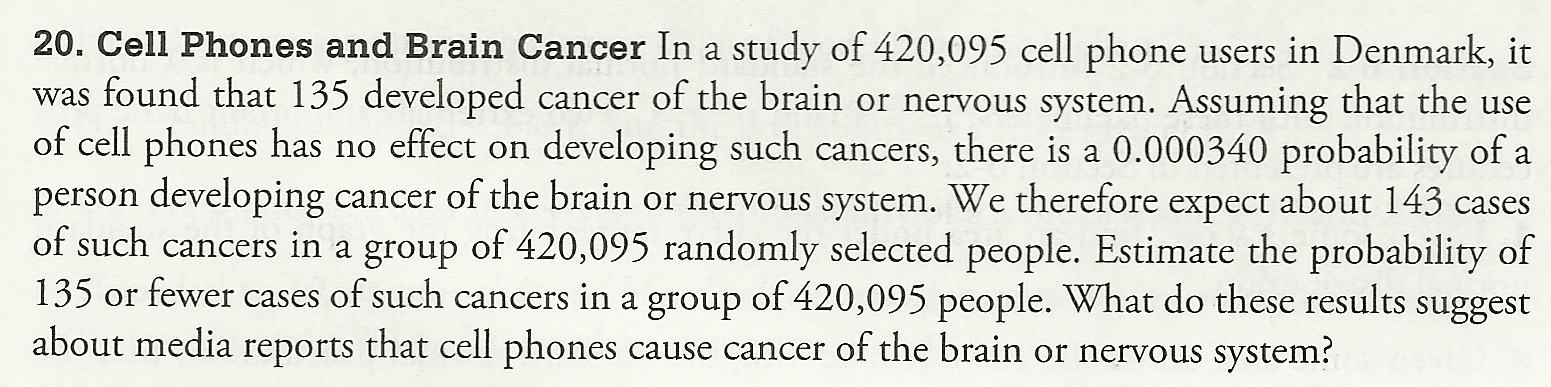
\includegraphics[scale=.7]{./triola3.png}
  \end{figure}
\end{frame}

\begin{frame}
  \frametitle{Word Problems III}
  \begin{figure}[h]
    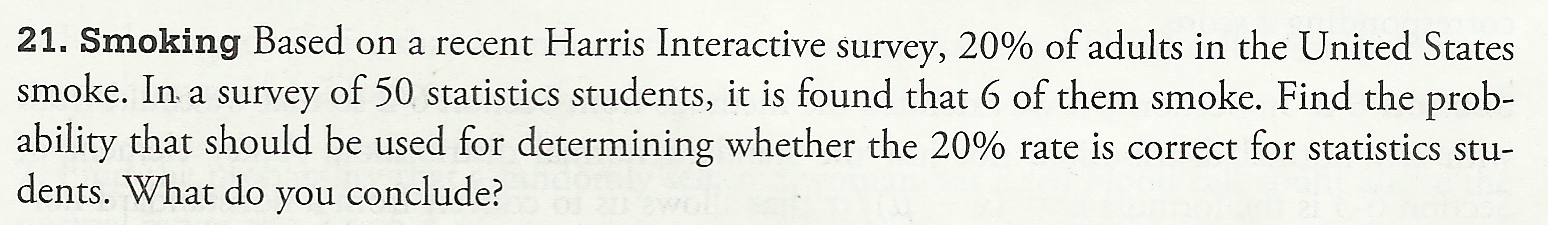
\includegraphics[scale=.7]{./triola4.png}
  \end{figure}
  \begin{figure}[h]
    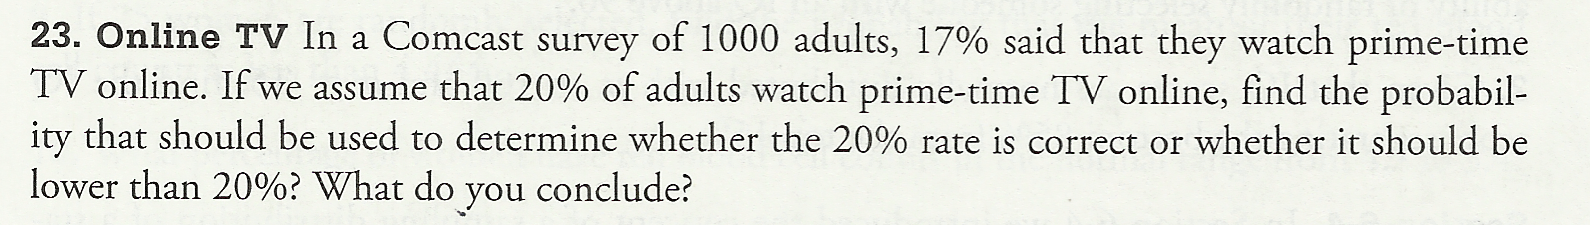
\includegraphics[scale=.7]{./triola5.png}
  \end{figure}
  \begin{figure}[h]
    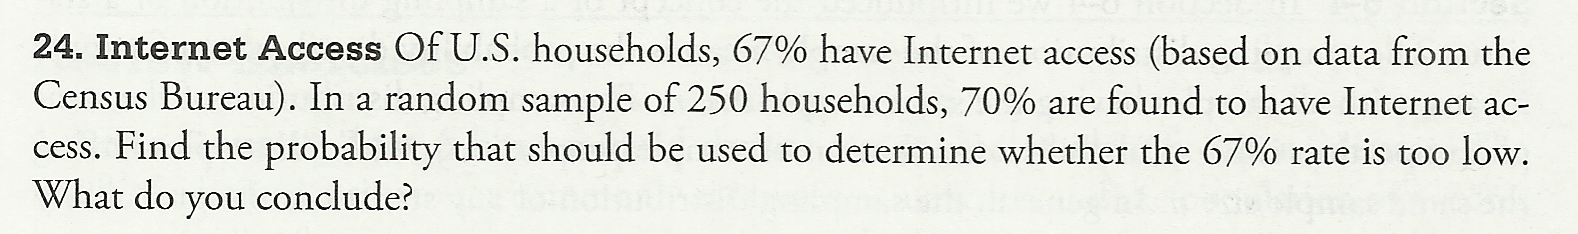
\includegraphics[scale=.7]{./triola6.png}
  \end{figure}
\end{frame}

\begin{frame}
  \frametitle{End of Lesson}
Next Lesson: Right Spherical Trigonometry
\end{frame}

\end{document}
